\documentclass[aspectratio=169,11pt]{beamer}

% ---------- Minimal, safe packages ----------
\usepackage[T1]{fontenc}
\usepackage[utf8]{inputenc}
\usepackage{lmodern}
\usepackage{graphicx}
\usepackage{booktabs}
\usepackage{xcolor}
\usepackage{tikz}
\usepackage{listings}
\usepackage{xcolor}
\usepackage{multirow}

\lstset{
  basicstyle={\ttfamily\fontsize{6.0}{5.3}\selectfont},
  breaklines=true,
  columns=fullflexible,
  frame=single,
  keepspaces=true,
  showstringspaces=false,
  aboveskip=0pt,
  belowskip=0pt,
  xleftmargin=0pt,
  xrightmargin=0pt,
  framexleftmargin=1mm,
  framexrightmargin=1mm
}

\usetikzlibrary{arrows.meta,positioning,shapes.geometric,fit}

% ---------- Theme ----------
\usetheme{Madrid}
\usecolortheme{default}
\setbeamertemplate{navigation symbols}{}
\setbeamertemplate{footline}[frame number]

% ---------- Colors ----------
\definecolor{GBlue}{RGB}{35,92,180}
\definecolor{GGreen}{RGB}{15,135,95}
\definecolor{GOrange}{RGB}{230,126,34}
\definecolor{GGray}{RGB}{245,245,245}
\definecolor{GDark}{RGB}{55,55,55}

\setbeamercolor{title}{fg=GBlue}
\setbeamercolor{frametitle}{fg=white,bg=GBlue}
\setbeamercolor{structure}{fg=GBlue}

% ---------- Helper boxes ----------
\newcommand{\placeholder}[1]{%
  \begin{center}
  \fbox{%
    \begin{minipage}[c][0.36\textheight][c]{0.88\linewidth}
      \centering\color{GDark}\Large #1
    \end{minipage}%
  }
  \end{center}
}

\newcommand{\smallplaceholder}[1]{%
  \fbox{%
    \begin{minipage}[c][0.20\textheight][c]{0.92\linewidth}
      \centering\color{GDark} #1
    \end{minipage}%
  }
}

\title{G$^3$VLA: Geometric Inductive Bias for Vision-Language-Action Models}
\author{Anonymous Authors}
\institute{}
\date{CoRL 2026 Overview Video}

\begin{document}

% =========================================================
% Slide 1
% =========================================================
\begin{frame}[plain]
  \vspace{1.0cm}

  \begin{center}
    {\Huge\bfseries\color{GBlue} G$^3$VLA}

    \vspace{0.45cm}

    {\Large\bfseries Geometric Inductive Bias for Vision-Language-Action Models}

    \vspace{0.35cm}

\begin{center}
  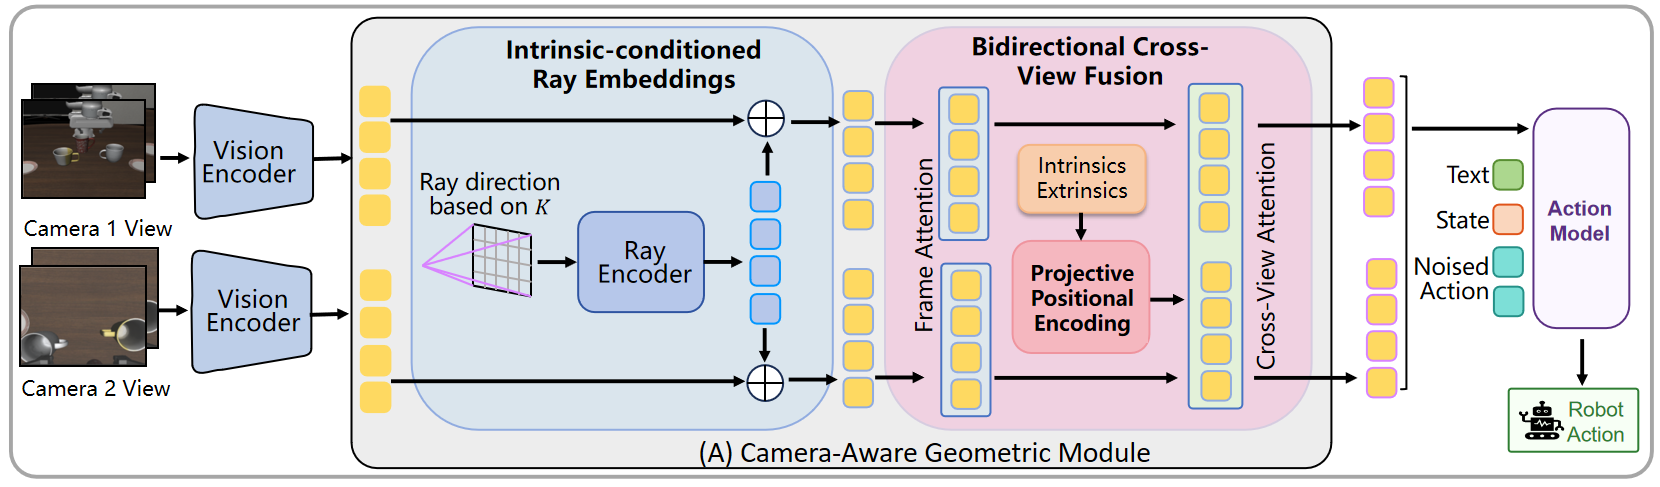
\includegraphics[width=0.92\linewidth]{imgs/g3vla_overview_module.png}
\end{center}

    \vfill

    {\normalsize CoRL 2026 Overview Video}
  \end{center}
\end{frame}

% =========================================================
% Slide 2
% =========================================================
\begin{frame}
  \frametitle{Motivation: Semantics vs. Geometry}

  \vspace{0.02cm}

  \begin{columns}[T,onlytextwidth]
    % -----------------------------------------------------
    % Left column
    % -----------------------------------------------------
    \begin{column}{0.47\textwidth}
      \textbf{Pretrained VLA Policies}

      \vspace{0.08cm}
      \begin{center}
        \fbox{%
          \begin{minipage}[c][0.065\textheight][c]{0.92\linewidth}
            \centering
            \small
            RGB + language $\rightarrow$ VLA $\rightarrow$ action
          \end{minipage}%
        }
      \end{center}

      \vspace{0.10cm}

      {\small
      \renewcommand{\arraystretch}{1.18}
      \begin{tabular}{@{}p{0.25\linewidth}p{0.67\linewidth}@{}}
        \textbf{Examples} & RT-2, OpenVLA, $\pi_0$, $\pi_{0.5}$, GR00T \\
        \textbf{Pros}     & strong semantics; scalable VLM priors \\
        \textbf{Cons}     & 2D image tokens; implicit geometry
      \end{tabular}
      }
    \end{column}

    % -----------------------------------------------------
    % Right column
    % -----------------------------------------------------
    \begin{column}{0.47\textwidth}
      \textbf{Geometry-Centric Policies}

      \vspace{0.08cm}
      \begin{center}
        \fbox{%
          \begin{minipage}[c][0.065\textheight][c]{0.92\linewidth}
            \centering
            \small
            RGB-D / point cloud / voxel $\rightarrow$ 3D policy
          \end{minipage}%
        }
      \end{center}

      \vspace{0.10cm}

      {\small
      \renewcommand{\arraystretch}{1.18}
      \begin{tabular}{@{}p{0.25\linewidth}p{0.67\linewidth}@{}}
        \textbf{Examples} & PerAct, RVT, Act3D, 3D Diffuser Actor \\
        \textbf{Pros}     & explicit 3D structure; spatial precision \\
        \textbf{Cons}     & depth/3D representations; less plug-and-play
      \end{tabular}
      }
    \end{column}
  \end{columns}

  \vspace{0.28cm}

  \begin{center}
    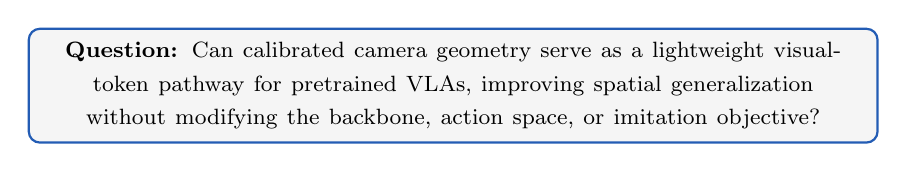
\begin{tikzpicture}
      \node[
        rounded corners,
        draw=GBlue,
        thick,
        fill=GGray,
        text width=0.86\linewidth,
        align=center,
        inner sep=5pt
      ] {
        \footnotesize
        \textbf{Question:}
        Can calibrated camera geometry serve as a lightweight visual-token pathway for pretrained VLAs,
        improving spatial generalization without modifying the backbone, action space, or imitation objective?
      };
    \end{tikzpicture}
  \end{center}

\end{frame}

% =========================================================
% Slide 3
% =========================================================
\begin{frame}
  \frametitle{Core Idea: Inject Geometry Before Action Prediction}

  \vspace{0.35cm}

  \begin{center}
  \resizebox{0.96\linewidth}{!}{%
  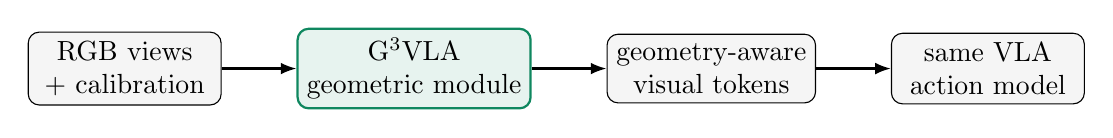
\begin{tikzpicture}[
    node distance=0.95cm,
    block/.style={
      draw,
      rounded corners,
      minimum width=2.45cm,
      minimum height=0.85cm,
      align=center,
      fill=GGray
    },
    gblock/.style={
      draw=GGreen,
      rounded corners,
      minimum width=2.75cm,
      minimum height=0.9cm,
      align=center,
      fill=GGreen!10,
      thick
    },
    arrow/.style={-{Latex[length=2mm]}, thick}
  ]
    \node[block] (rgb) {RGB views\\+ calibration};
    \node[gblock, right=of rgb] (geom) {G$^3$VLA\\geometric module};
    \node[block, right=of geom] (tokens) {geometry-aware\\visual tokens};
    \node[block, right=of tokens] (action) {same VLA\\action model};

    \draw[arrow] (rgb) -- (geom);
    \draw[arrow] (geom) -- (tokens);
    \draw[arrow] (tokens) -- (action);
  \end{tikzpicture}%
  }
  \end{center}

  \vspace{0.75cm}

  \begin{columns}[T,onlytextwidth]
    % -----------------------------------------------------
    % Left card
    % -----------------------------------------------------
    \begin{column}{0.48\textwidth}
      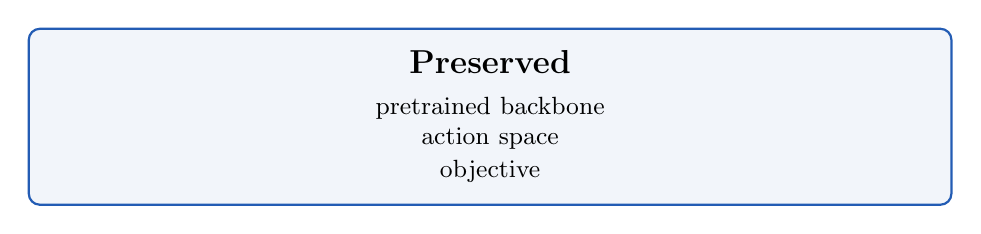
\begin{tikzpicture}
        \node[
          rounded corners,
          draw=GBlue,
          thick,
          fill=GBlue!6,
          text width=0.92\linewidth,
          align=center,
          inner sep=8pt
        ] {
          {\large\textbf{Preserved}}\\[0.35em]
          \small
          pretrained backbone\\
          action space\\
          objective
        };
      \end{tikzpicture}
    \end{column}

    % -----------------------------------------------------
    % Right card
    % -----------------------------------------------------
    \begin{column}{0.48\textwidth}
      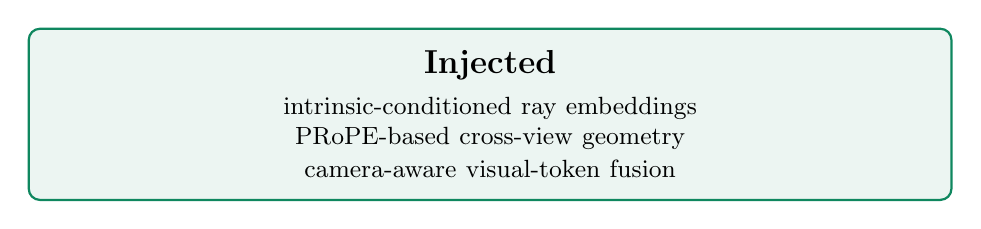
\begin{tikzpicture}
        \node[
          rounded corners,
          draw=GGreen,
          thick,
          fill=GGreen!8,
          text width=0.92\linewidth,
          align=center,
          inner sep=8pt
        ] {
          {\large\textbf{Injected}}\\[0.35em]
          \small
          intrinsic-conditioned ray embeddings\\
          PRoPE-based cross-view geometry\\
          camera-aware visual-token fusion
        };
      \end{tikzpicture}
    \end{column}
  \end{columns}

  \vspace{0.45cm}

  \begin{center}
    {\small\color{GDark}
    Geometry enters through the visual-token stream, before action generation.}
  \end{center}

\end{frame}
% =========================================================
% Slide 4
% =========================================================
\begin{frame}
  \frametitle{Methods}

  \vspace{0.10cm}

  \begin{columns}[T,onlytextwidth]
    % -----------------------------------------------------
    % Card 1
    % -----------------------------------------------------
    \begin{column}{0.30\textwidth}
      \begin{block}{1. Ray embeddings}
        \begin{center}
          \fbox{%
            \begin{minipage}[c][0.105\textheight][c]{0.92\linewidth}
              \centering
              \scriptsize
              $\tilde{\mathbf r}^{v}(\mathbf u)=(K^v)^{-1}\mathbf u$\\[0.25em]
              $R^v(x,y)=\tilde{\mathbf r}^{v}_{1:2}$
            \end{minipage}%
          }
        \end{center}

        \vspace{0.08cm}
        {\scriptsize
        Tags each patch with its calibrated viewing direction.
        }
      \end{block}
    \end{column}

    \hfill

    % -----------------------------------------------------
    % Card 2
    % -----------------------------------------------------
    \begin{column}{0.30\textwidth}
      \begin{block}{2. PRoPE}
        \begin{center}
          \fbox{%
            \begin{minipage}[c][0.105\textheight][c]{0.92\linewidth}
              \centering
              \scriptsize
              projective positional encoding\\[0.25em]
              $\{K^v,T^v\}_{v=1}^{V}$
            \end{minipage}%
          }
        \end{center}

        \vspace{0.08cm}
        {\scriptsize
        Gives attention camera-calibrated cross-view relations.
        }
      \end{block}
    \end{column}

    \hfill

    % -----------------------------------------------------
    % Card 3
    % -----------------------------------------------------
    \begin{column}{0.30\textwidth}
      \begin{block}{3. Cross-view fusion}
        \begin{center}
          \fbox{%
            \begin{minipage}[c][0.105\textheight][c]{0.92\linewidth}
              \centering
              \scriptsize
              Frame Attention\\[-0.1em]
              $+$ Cross-View Attention\\[0.25em]
              $H=\mathrm{Fusion}_{\psi}(Z;\{K^v,T^v\})$
            \end{minipage}%
          }
        \end{center}

        \vspace{0.08cm}
        {\scriptsize
        Lets camera streams exchange geometric context.
        }
      \end{block}
    \end{column}
  \end{columns}

  \vspace{0.28cm}

  \begin{center}
    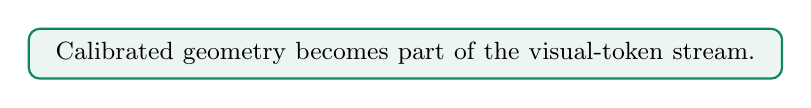
\begin{tikzpicture}
      \node[
        rounded corners,
        draw=GGreen,
        thick,
        fill=GGreen!8,
        text width=0.76\linewidth,
        align=center,
        inner sep=5pt
      ] {
        \small
        Calibrated geometry becomes part of the visual-token stream.
      };
    \end{tikzpicture}
  \end{center}

\end{frame}

% =========================================================
% Slide 4.1
% =========================================================
\begin{frame}[fragile]
  \frametitle{Method 1: Intrinsic-conditioned Ray Embeddings}

  \vspace{-0.15cm}

  \begin{columns}[T,onlytextwidth]

    % -----------------------------------------------------
    % Left: code
    % -----------------------------------------------------
    \begin{column}{0.52\textwidth}
      {\scriptsize\textbf{Implementation: construct ray embeddings from intrinsics}}

      \vspace{0.06cm}

      \begin{lstlisting}[language=Python]
if ray_enc_type:
    vision_patch_size = vlm_config_hf.vision_config.patch_size
    vision_dim = vlm_config_hf.vision_config.hidden_size
    self.ray_embed = PatchEmbed(
        patch_size=vision_patch_size,
        in_chans=2,
        embed_dim=vision_dim,
    )
    nn.init.constant_(self.ray_embed.proj.weight, 0)
    nn.init.constant_(self.ray_embed.proj.bias, 0)
...
if self.ray_enc_type and cam_intr is not None:
    ray_dtype = self.ray_embed.proj.weight.dtype
    K_stack = []
    for cam_key in cam_keys:
        K_per = cam_intr.get(cam_key)
        if K_per is None:
            K_per = torch.eye(
                3, device=device, dtype=ray_dtype
            )[None].expand(B, -1, -1)
        K_stack.append(K_per)
    cam_intr_stacked = torch.stack(K_stack, dim=1)
    pix = torch.from_numpy(
        get_pixel(H, W).T.reshape(H, W, 3)
    ).to(device=device, dtype=ray_dtype)
    pix = pix[None].expand(B, -1, -1, -1)
    K_inv = torch.linalg.inv(
        cam_intr_stacked.float()
    ).to(ray_dtype)
    rays = torch.einsum(
        "bvij,bhwj->bvhwi", K_inv, pix
    )[..., :2]
    ray_emb_bv = self.ray_embed(
        rays.reshape(B * V, H, W, 2)
            .permute(0, 3, 1, 2))
      \end{lstlisting}
    \end{column}

    \hfill

    % -----------------------------------------------------
    % Right: figure only
    % -----------------------------------------------------
    \begin{column}{0.44\textwidth}
      {\scriptsize\textbf{Visualization: patch tokens as calibrated rays}}

      \vspace{0.06cm}

      \begin{center}
        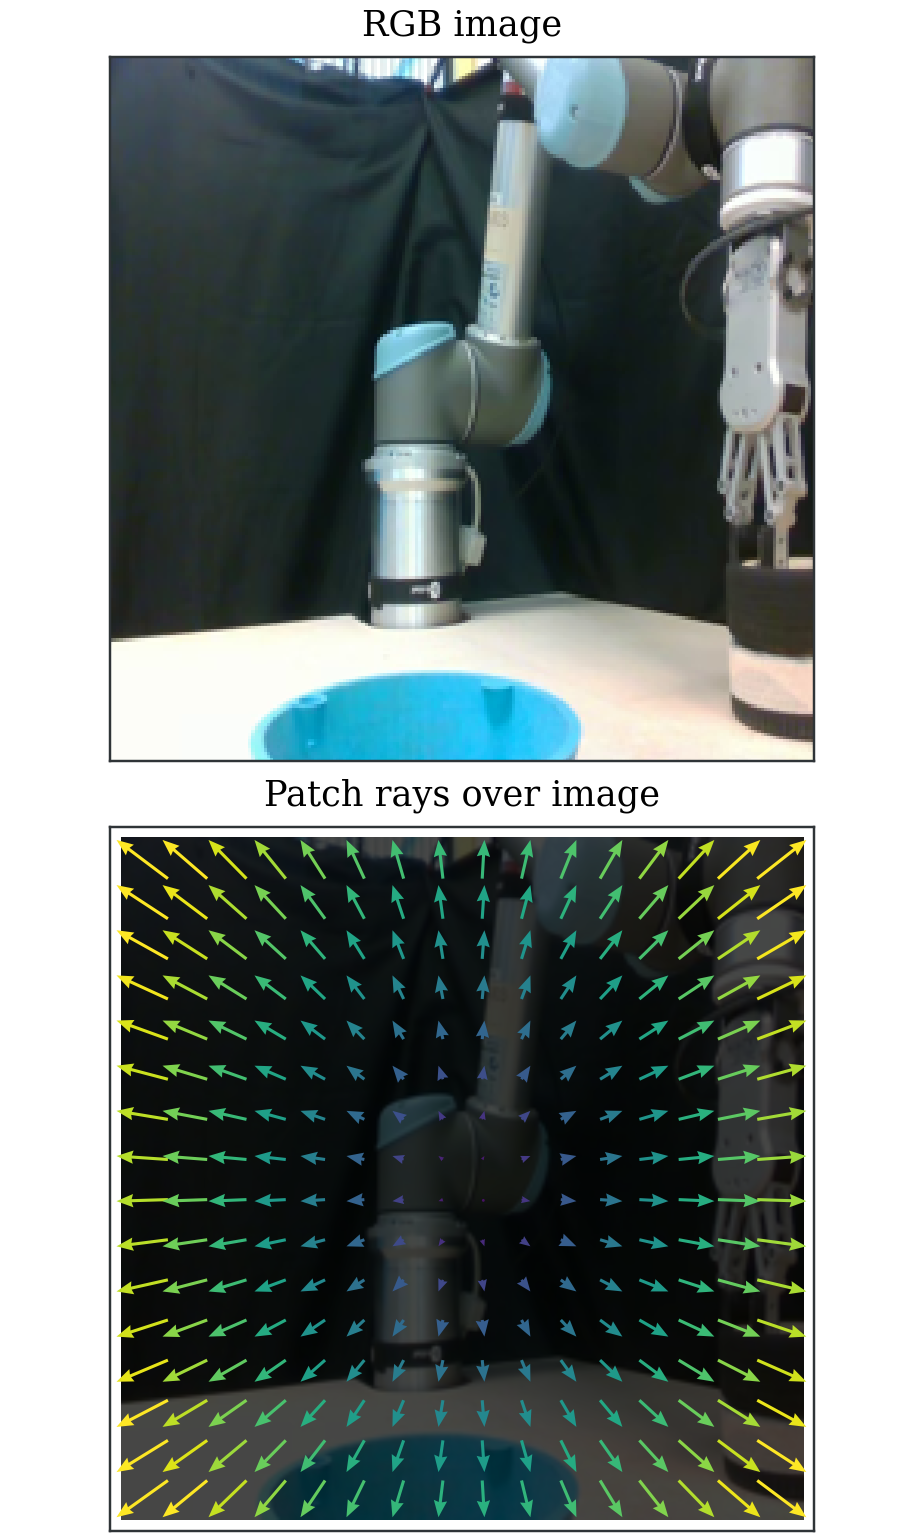
\includegraphics[width=1\linewidth,height=0.8\textheight,keepaspectratio]{imgs/ray_emb.png}
      \end{center}
    \end{column}

  \end{columns}
\end{frame}

% =========================================================
% Slide 4.2
% =========================================================
\begin{frame}[fragile]
  \frametitle{Method 2: PRoPE}

  \vspace{-0.15cm}

  \begin{columns}[T,onlytextwidth]

    % -----------------------------------------------------
    % Left: code
    % -----------------------------------------------------

    \begin{column}{0.52\textwidth}
      {\scriptsize\textbf{Implementation: prepare PRoPE attention transforms}}

      \vspace{0.06cm}

      \begin{lstlisting}[language=Python]
def prepare_apply_fns(head_dim: int,
      viewmats: torch.Tensor, Ks: Optional[torch.Tensor],
      patches_x: int, patches_y: int,
      image_width: int, image_height: int,
      freq_base: float = 100.0,) -> Tuple[Callable, Callable, Callable]:
      ...
      if Ks is not None:
          Ks_norm = torch.zeros_like(Ks)
          ...
          P = torch.einsum("...ij,...jk->...ik", _lift_K(Ks_norm), viewmats)
          P_T = P.transpose(-1, -2)
          P_inv = torch.einsum("...ij,...jk->...ik", _invert_SE3(viewmats), _lift_K(_invert_K(Ks_norm)))
      else:
          ...
      coeffs_x = _rope_precompute_coeffs(..., feat_dim=head_dim // 4)
      coeffs_y = _rope_precompute_coeffs(..., feat_dim=head_dim // 4)
      transforms_q = [(partial(_apply_tiled_projmat, matrix=P_T), head_dim // 2),
          (partial(_rope_apply_coeffs, coeffs=coeffs_x), head_dim // 4),
          (partial(_rope_apply_coeffs, coeffs=coeffs_y), head_dim // 4),]
      transforms_kv = [(partial(_apply_tiled_projmat, matrix=P_inv), head_dim // 2), ...]
      transforms_o = [(partial(_apply_tiled_projmat, matrix=P), head_dim // 2), ...]
      return (partial(_apply_block_diagonal, func_size_pairs=transforms_q),
          partial(_apply_block_diagonal, func_size_pairs=transforms_kv),
          partial(_apply_block_diagonal, func_size_pairs=transforms_o),)
      \end{lstlisting}
    \end{column}

    \hfill

    % -----------------------------------------------------
    % Right: figure only
    % -----------------------------------------------------
    \begin{column}{0.44\textwidth}
      {\scriptsize\textbf{Visualization: projective positional encoding}}

      \vspace{0.06cm}

      \begin{center}
        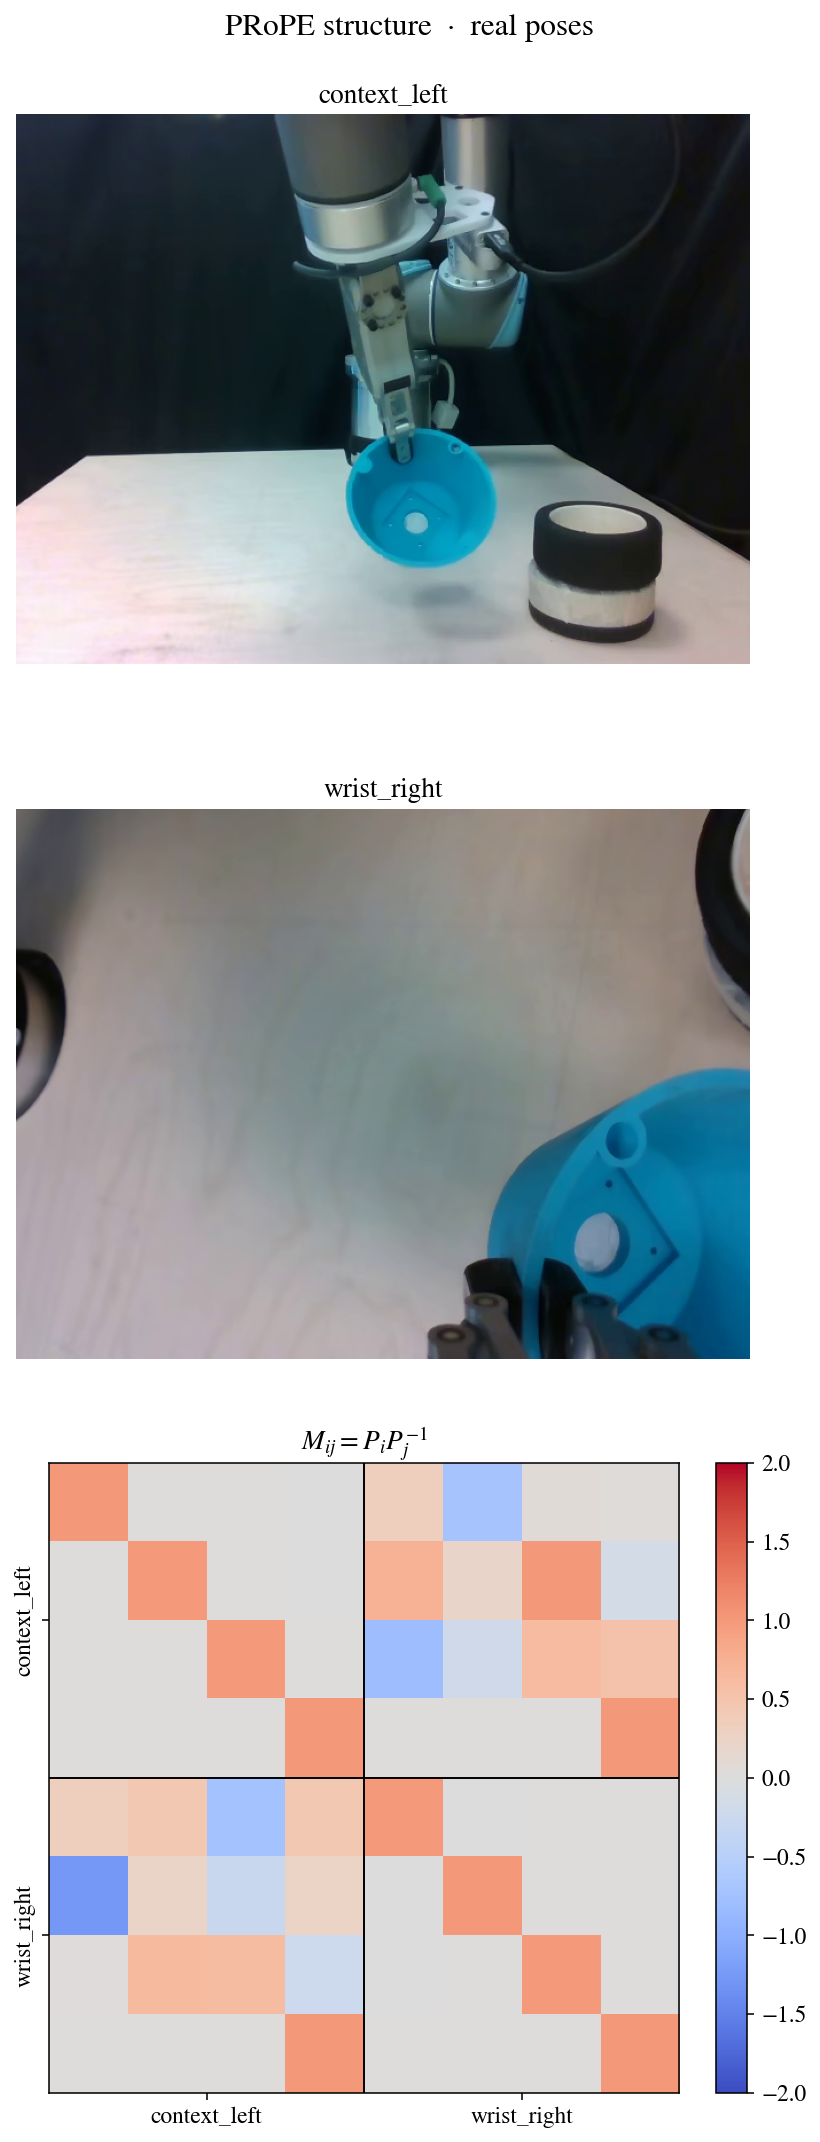
\includegraphics[width=1\linewidth,height=0.8\textheight,keepaspectratio]{imgs/PRoPE2.png}
      \end{center}
    \end{column}

  \end{columns}
\end{frame}

% =========================================================
% Slide 4.3
% =========================================================
\begin{frame}[fragile]
  \frametitle{Method 3: Cross-view Fusion}

  \vspace{-0.15cm}

  \begin{columns}[T,onlytextwidth]

    % -----------------------------------------------------
    % Left: code
    % -----------------------------------------------------
    \begin{column}{0.52\textwidth}
      {\scriptsize\textbf{Implementation: alternate frame and global attention}}

      \vspace{0.06cm}

      \begin{lstlisting}[language=Python]
for attn_type in self.aa_order:                       # e.g. "fg" -> frame, global, frame, global, ...
    if attn_type == "f":
        tokens = self._process_frame_attention(...,  frame_idx, ...)
        frame_idx += 1
    elif attn_type == "g":
        tokens = self._process_global_attention(..., global_idx, ...)
        # (PRoPE PoseInjectBlock optionally added here after a global block)
        global_idx += 1
return tokens.reshape(bsz, num_views, num_tokens, dim)
...
def _process_frame_attention(self, tokens, bsz, num_views, num_tokens, dim, layer_idx, pos, mask):
    # (B, V, T, D) -> (B*V, T, D): each view attends ONLY within itself
    tokens = tokens.reshape(bsz * num_views, num_tokens, dim)
    frame_mask = ~mask.reshape(bsz * num_views, num_tokens) if mask is not None else None
    return self.frame_blocks[layer_idx](tokens, pos=pos, attn_mask=frame_mask)

def _process_global_attention(self, tokens, bsz, num_views, num_tokens, dim, layer_idx, pos, mask):
    # (B, V, T, D) -> (B, V*T, D): all tokens of all views attend jointly (cross-view)
    tokens = tokens.reshape(bsz, num_views * num_tokens, dim)
    global_mask = ~mask.reshape(bsz, num_views * num_tokens) if mask is not None else None
    return self.global_blocks[layer_idx](tokens, pos=pos, attn_mask=global_mask)
      \end{lstlisting}
    \end{column}

    \hfill

    % -----------------------------------------------------
    % Right: figure only
    % -----------------------------------------------------
    \begin{column}{0.44\textwidth}
      {\scriptsize\textbf{Visualization: frame attention + cross-view fusion}}

      \vspace{0.06cm}

      \begin{center}
        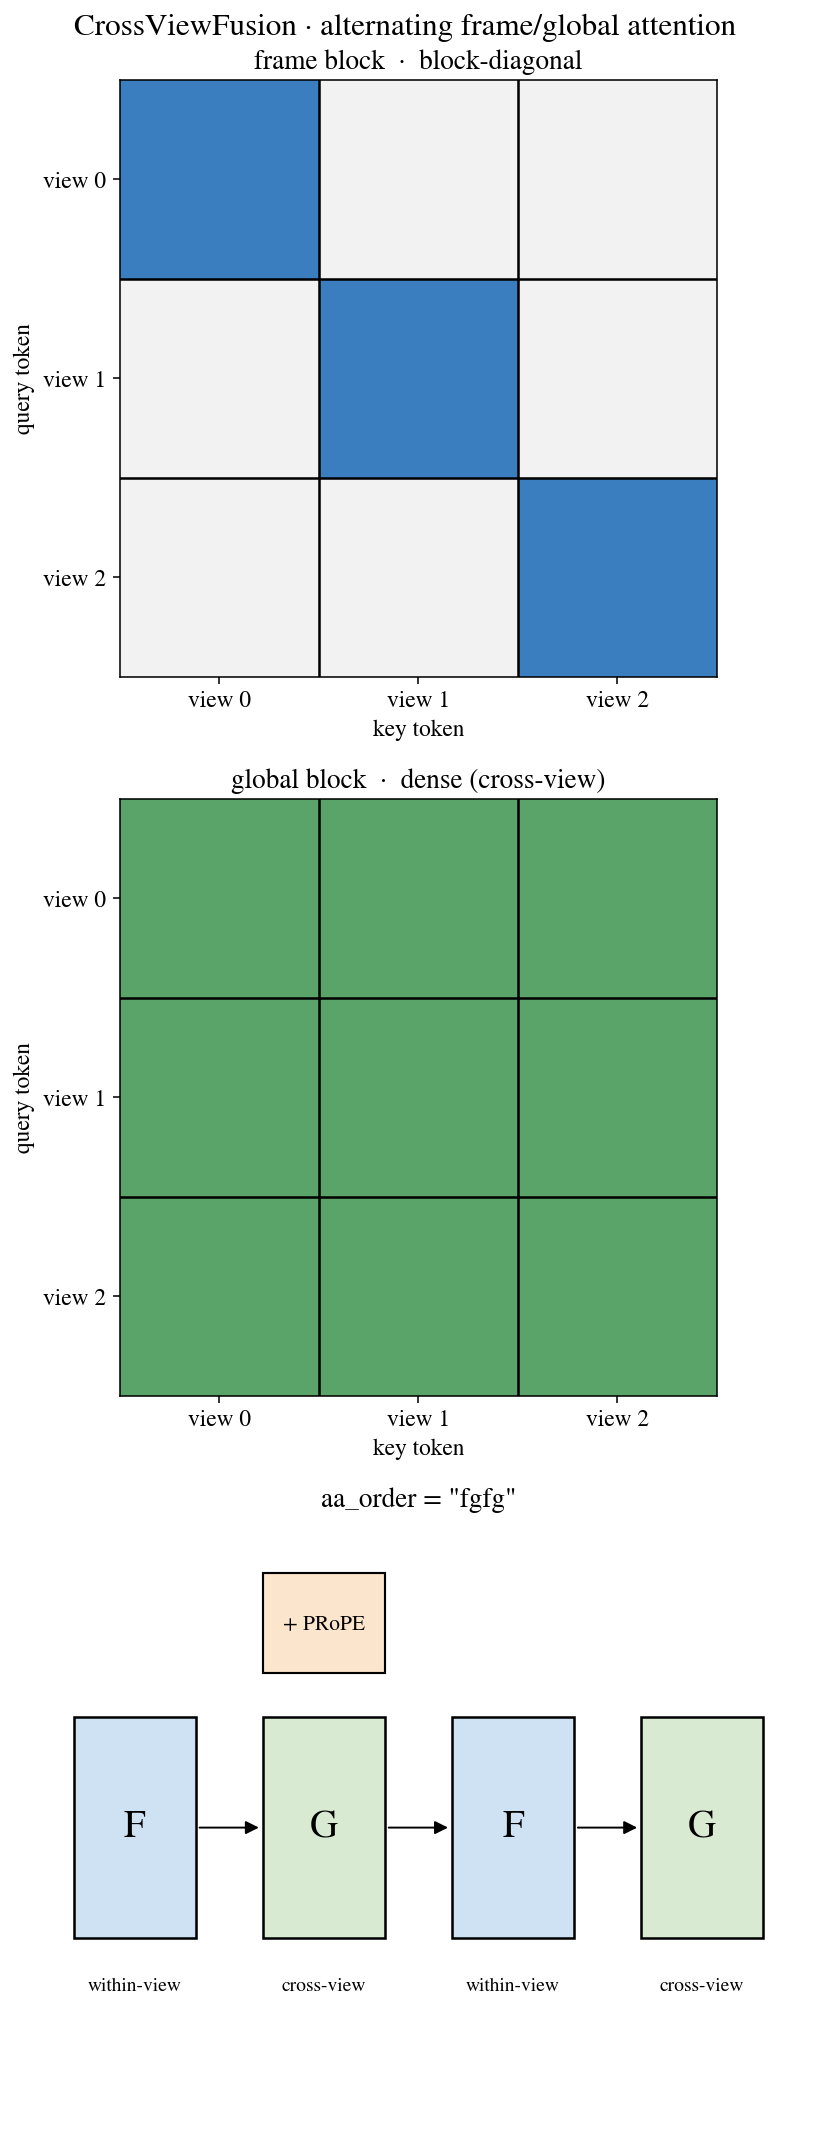
\includegraphics[width=1\linewidth,height=0.8\textheight,keepaspectratio]{imgs/Fusion.png}
      \end{center}
    \end{column}

  \end{columns}
\end{frame}

% =========================================================
% Slide 5
% =========================================================
\begin{frame}
  \frametitle{Training}

  \vspace{0.10cm}

  \begin{center}
    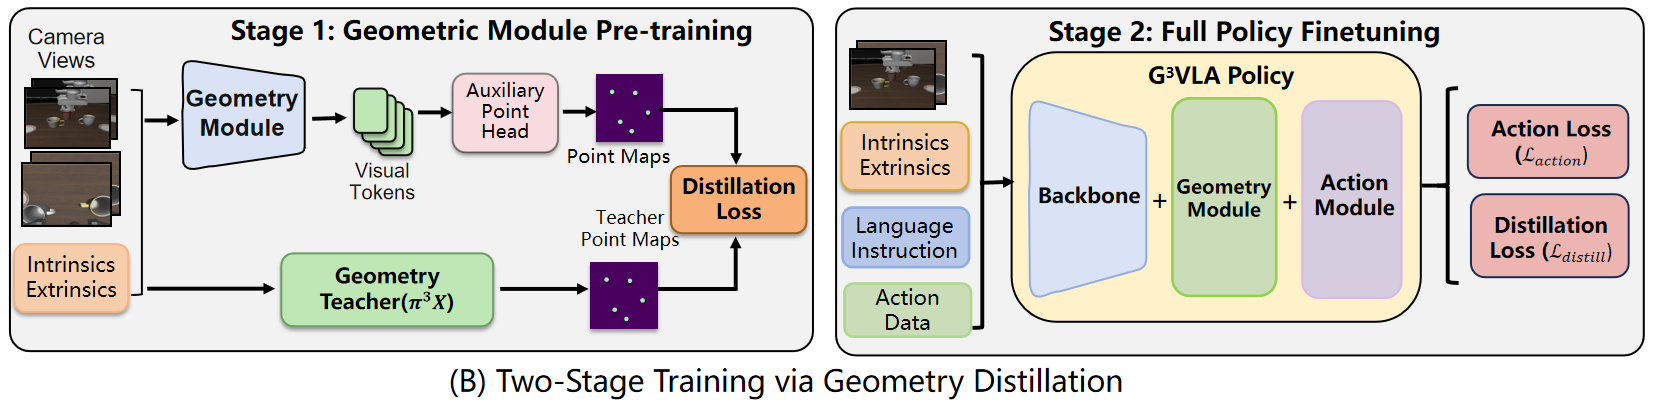
\includegraphics[
      width=0.96\linewidth,
      height=0.78\textheight,
      keepaspectratio
    ]{imgs/2-stages.png}
  \end{center}

\end{frame}

% =========================================================
% Slide 5.1
% =========================================================
\begin{frame}
  \frametitle{Supervision Source}

  \vspace{0.10cm}

  \begin{center}
    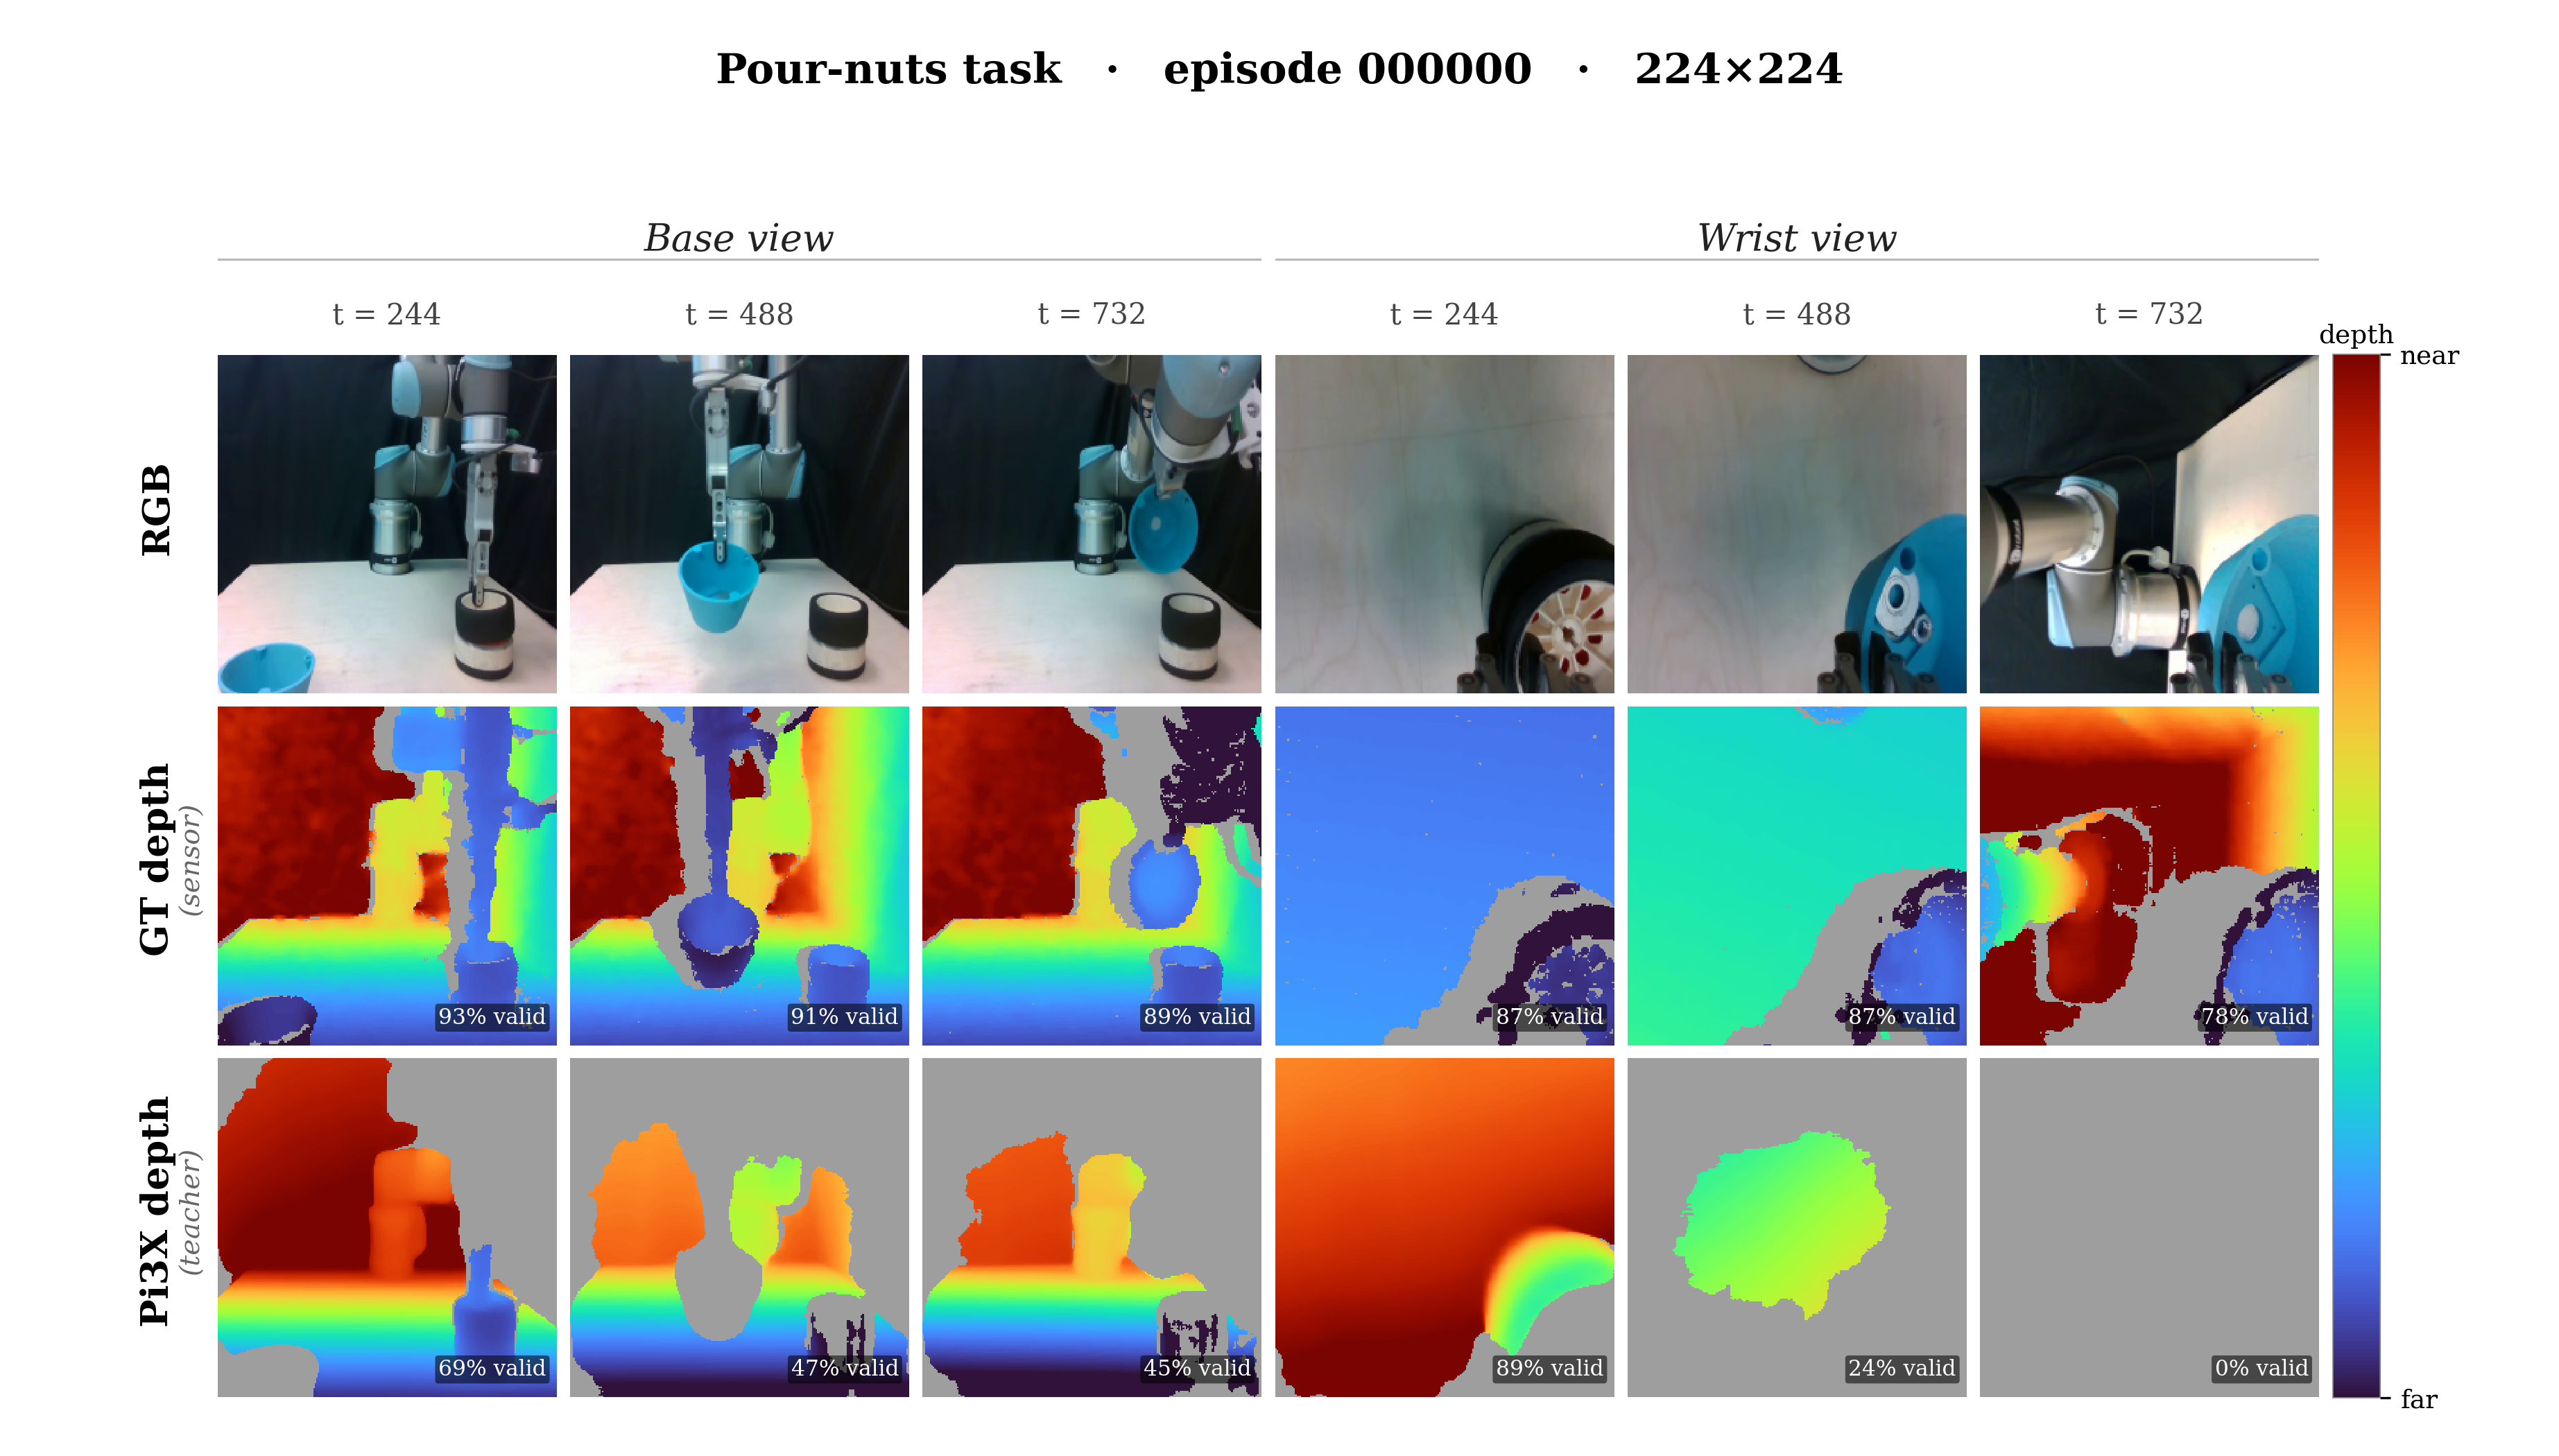
\includegraphics[
      width=0.88\linewidth,
      height=1\textheight,
      keepaspectratio
    ]{imgs/supervision.png}
  \end{center}

\end{frame}

% =========================================================
% Slide 6
% =========================================================
\begin{frame}
  \frametitle{Results: Simulation Benchmarks}

  \vspace{-0.05cm}

  \begin{columns}[T,onlytextwidth]

    % -----------------------------------------------------
    % Left: pi0 main results
    % -----------------------------------------------------
    \begin{column}{0.49\textwidth}

      \textbf{\small $\pi_0$ on LIBERO}

      \vspace{0.06cm}

      \begin{table}
      \centering
      \scriptsize
      \renewcommand{\arraystretch}{1.12}
      \begin{tabular}{lcccc}
        \toprule
        \textbf{Suite} & \textbf{Base} & \textbf{$\pi^3$X} & \textbf{GT} & \textbf{Gain} \\
        \midrule
        Goal    & 87.4 & 88.4 & 88.4 & +1.0 \\
        Spatial & 85.2 & 88.6 & 89.2 & +4.0 \\
        Object  & 89.4 & 93.4 & 94.4 & +5.0 \\
        L-10    & 76.5 & 77.6 & 80.4 & +3.9 \\
        Avg.    & 84.6 & 87.0 & 88.1 & +3.5 \\
        \bottomrule
      \end{tabular}
      \end{table}

      \vspace{0.18cm}

      \textbf{\small $\pi_0$ on broader simulation benchmarks}

      \vspace{0.06cm}

      \begin{table}
      \centering
      \scriptsize
      \renewcommand{\arraystretch}{1.12}
      \begin{tabular}{lccc}
        \toprule
        \textbf{Benchmark} & \textbf{Base} & \textbf{$\pi^3$X} & \textbf{GT} \\
        \midrule
        RoboCasa24  & 34.2 & 36.5 & 37.1 \\
        RoboTwin2.0 & 44.0 & 41.0 & 49.0 \\
        \bottomrule
      \end{tabular}
      \end{table}

    \end{column}

    \hfill

    % -----------------------------------------------------
    % Right: backbone generalization
    % -----------------------------------------------------
    \begin{column}{0.49\textwidth}

      \textbf{\small $\pi_{0.5}$ on LIBERO}

      \vspace{0.06cm}

      \begin{table}
      \centering
      \scriptsize
      \renewcommand{\arraystretch}{1.12}
      \begin{tabular}{lccc}
        \toprule
        \textbf{Suite} & \textbf{Official} & \textbf{Reprod.} & \textbf{G$^3$VLA} \\
        \midrule
        Spatial & 98.0 & 98.8 & 98.2 \\
        Object  & 99.0 & 98.4 & 99.0 \\
        Goal    & 98.2 & 94.4 & 98.0 \\
        L-10    & 91.4 & 91.8 & 92.8 \\
        Avg.    & 96.7 & 95.9 & 97.0 \\
        \bottomrule
      \end{tabular}
      \end{table}

      \vspace{0.18cm}

      \textbf{\small GR00T 1.5 on LIBERO}

      \vspace{0.06cm}

      \begin{table}
      \centering
      \scriptsize
      \renewcommand{\arraystretch}{1.12}
      \begin{tabular}{lccc}
        \toprule
        \textbf{Suite} & \textbf{Base} & \textbf{GT} & \textbf{$\pi^3$X} \\
        \midrule
        Spatial & 96.6 & 94.2 & 96.6 \\
        Object  & 97.0 & 97.0 & 99.0 \\
        Goal    & 95.4 & 94.2 & 95.8 \\
        L-10    & 90.6 & 92.6 & 89.6 \\
        Avg.    & 94.9 & 94.5 & 95.25 \\
        \bottomrule
      \end{tabular}
      \end{table}

    \end{column}

  \end{columns}

  \vspace{0.05cm}

  \begin{center}
    {\tiny Success rate (\%).}
  \end{center}

\end{frame}

% =========================================================
% Slide 7
% =========================================================
\begin{frame}
  \frametitle{Results: Real-robot Benchmarks}

  \vspace{-0.10cm}

  % -----------------------------------------------------
  % Pick-and-Place Test Tube
  % -----------------------------------------------------
  \begin{table}
  \centering
  \tiny
  \renewcommand{\arraystretch}{1.10}
  \setlength{\tabcolsep}{2.4pt}
  \textbf{Pick-and-Place Test Tube}
  \vspace{0.04cm}

  \resizebox{0.96\linewidth}{!}{%
  \begin{tabular}{c|ccc|ccc|ccc|ccc}
    \toprule
    \multirow{2}{*}{\textbf{Chkpt.}}
    & \multicolumn{3}{c|}{$\pi_0$}
    & \multicolumn{3}{c|}{G$^3$VLA $(\pi_0+\pi^3X)$}
    & \multicolumn{3}{c|}{$\pi_{0.5}$}
    & \multicolumn{3}{c}{G$^3$VLA $(\pi_{0.5}+\pi^3X)$} \\
    & ID & OOD & Overall
    & ID & OOD & Overall
    & ID & OOD & Overall
    & ID & OOD & Overall \\
    \midrule
    20K & 75.0 & 50.0 & 60.0 & 75.0 & 33.3 & 50.0 & 50.0 & 41.7 & 45.0 & 62.5 & 33.3 & 45.0 \\
    25K & 62.5 & 41.7 & 50.0 & 75.0 & 41.7 & 55.0 & 37.5 & 25.0 & 30.0 & 50.0 & 50.0 & 50.0 \\
    30K & 75.0 & 58.3 & 65.0 & 75.0 & 58.3 & 65.0 & 37.5 & 41.7 & 40.0 & 62.5 & 58.3 & 60.0 \\
    \bottomrule
  \end{tabular}%
  }
  \end{table}

  \vspace{0.12cm}

  % -----------------------------------------------------
  % Pouring Nut
  % -----------------------------------------------------
  \begin{table}
  \centering
  \tiny
  \renewcommand{\arraystretch}{1.10}
  \setlength{\tabcolsep}{2.4pt}
  \textbf{Pouring Nut}
  \vspace{0.04cm}

  \resizebox{0.96\linewidth}{!}{%
  \begin{tabular}{c|ccc|ccc|ccc|ccc}
    \toprule
    \multirow{2}{*}{\textbf{Chkpt.}}
    & \multicolumn{3}{c|}{$\pi_0$}
    & \multicolumn{3}{c|}{G$^3$VLA $(\pi_0+\mathrm{GT})$}
    & \multicolumn{3}{c|}{$\pi_{0.5}$}
    & \multicolumn{3}{c}{G$^3$VLA $(\pi_{0.5}+\mathrm{GT})$} \\
    & ID & OOD & Overall
    & ID & OOD & Overall
    & ID & OOD & Overall
    & ID & OOD & Overall \\
    \midrule
    20K & 100.0 & 70.8 & 82.5 & 100.0 & 83.3 & 90.0 & 93.75 & 66.7 & 77.5 & 93.75 & 70.8 & 80.0 \\
    25K & 100.0 & 75.0 & 85.0 & 100.0 & 87.5 & 92.5 & 100.0 & 66.7 & 80.0 & 87.50 & 79.2 & 82.5 \\
    \bottomrule
  \end{tabular}%
  }
  \end{table}

  \vspace{0.05cm}

  \begin{center}
    {\tiny Success rate / score (\%). ID = seen camera views; OOD = unseen camera views.}
  \end{center}

\end{frame}

% =========================================================
% Slide 8
% =========================================================
\begin{frame}
  \frametitle{Conclusion}

  \vspace{0.55cm}

  % -----------------------------------------------------
  % Block 1: short takeaway / conclusion
  % -----------------------------------------------------
  \begin{center}
    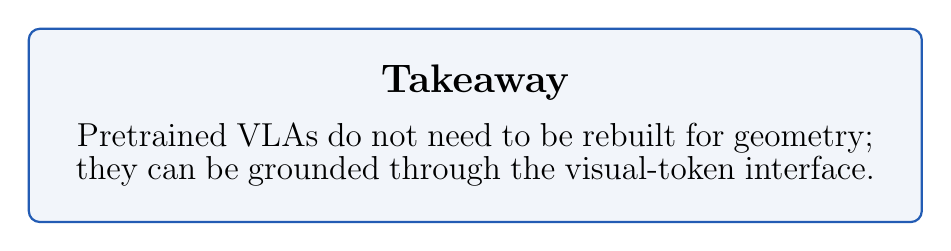
\begin{tikzpicture}
      \node[
        rounded corners,
        draw=GBlue,
        thick,
        fill=GBlue!6,
        text width=0.86\linewidth,
        align=center,
        inner sep=13pt
      ] {
        {\Large\textbf{Takeaway}}\\[0.55em]
        {\large
        Pretrained VLAs do not need to be rebuilt for geometry;\\
        they can be grounded through the visual-token interface.
        }
      };
    \end{tikzpicture}
  \end{center}

  \vspace{0.55cm}

  % -----------------------------------------------------
  % Block 2: restating the model
  % -----------------------------------------------------
  \begin{center}
    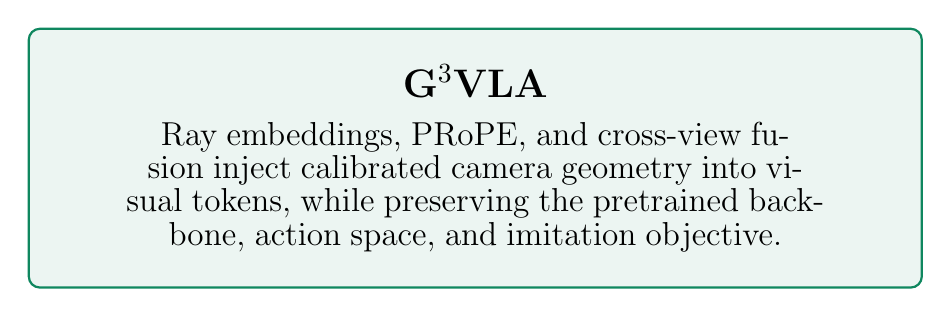
\begin{tikzpicture}
      \node[
        rounded corners,
        draw=GGreen,
        thick,
        fill=GGreen!8,
        text width=0.86\linewidth,
        align=center,
        inner sep=13pt
      ] {
        {\Large\textbf{G$^3$VLA}}\\[0.55em]
        {\large
        Ray embeddings, PRoPE, and cross-view fusion inject calibrated camera geometry
        into visual tokens, while preserving the pretrained backbone,
        action space, and imitation objective.
        }
      };
    \end{tikzpicture}
  \end{center}

\end{frame}

\end{document}

